\documentclass[12pt]{article}

% packages
\usepackage[margin=1in]{geometry}
\usepackage[labelfont=it, justification=centering]{caption}
\usepackage{subcaption}
\usepackage{framed}
\usepackage[table]{xcolor}
\usepackage{colortbl, multirow}
\usepackage{amsmath,amsthm,amssymb,wasysym}
\usepackage{mathrsfs, mathtools}
\usepackage{tikz,pgf,pgfplots}
\usetikzlibrary{arrows, angles, quotes, decorations.pathreplacing, math, patterns, calc}
\usepackage{graphicx}

% custom commands
\newcommand{\N}{\mathbb{N}}
\newcommand{\Z}{\mathbb{Z}}
\newcommand{\I}{\mathbb{I}}
\newcommand{\R}{\mathbb{R}}
\newcommand{\Q}{\mathbb{Q}}
\newcommand{\p}{^{\prime}}
\newcommand{\powerset}{\raisebox{.15\baselineskip}{\Large\ensuremath{\wp}}}
\DeclarePairedDelimiter{\ceil}{\lceil}{\rceil}
\DeclarePairedDelimiter\floor{\lfloor}{\rfloor}

 
\begin{document}
 
\title{Pigeonhole\\
    \large MATH CS 101B Problem Solving II}
\author{Harry Coleman}
\date{January 14, 2020}

\maketitle

\section*{Problem 12}
\fbox{
    \parbox{\textwidth} {
        Show that if $n+ 1$ integers are chosen from the set $\{1, 2, ..., 2n\}$, then there are always two which differ by 1.
    }
}
\\

It is assumed that all chosen integers are distinct from one another; if this were not the case, then all chosen integers could be equal and any two would differ by zero. In the given set, consider the pairs of integers that differ by 1 and have the lesser odd\textemdash that is, 
\[(1,2),(3,4),(5,6),\dots,(2n-1,2n).\]
The given set contains the integers 1 through $2n$, so there are $n$ of these pairs. If $n+1$ distinct integers are chosen, then at least two must be in the same pair, and therefore differ by 1.


\newpage
\section*{Problem 13}
\fbox{
    \parbox{\textwidth} {
        In a room there are 10 people, none of whom are older than 60 (ages are given in whole numbers only) but each of whom is at least 1 year old. Prove that one can always find two groups of people (with no common person) the sum of whose ages is the same. Can 10 be replaced by a smaller number?
    }
}
\\

Let $X=\{x_1, \dots, x_{10}\}$ be the set of people in the room. The power set $\powerset(X)$ would represent the set of all possible subsets of the ten people. We now define for all $A\in\powerset(X)$, sum($A$) which gives the sum of all the ages of the people in $A$. Since we are only concerned with taking two disjoint groups of people, we'll only consider groups with between one and nine people. So we'll take
\[P = \powerset(X)\setminus\{\emptyset, X\}.\]
We can find the number of possible subsets of one to nine people by
\[|P| = |\powerset(X)|-2=2^{10}-2=1022.\]
Since each person is between 1 and 60 years old, for each of our subsets $A\in P$, we know 
\[1\leq\text{sum}(A)\leq60\cdot9=540.\]

With 1022 subsets of people, each taking on a sum from 1 to 540, there must be at least two different subsets of people which have the same sum.
\[\text{Let } A,B\in P \text{ with } A\ne B \text{ and sum}(A)=\text{sum}(B).\]
If $A$ and $B$ have a nonempty intersection (some people who are in both subsets), we consider each set with this intersection removed. So we let
\begin{align*}
    A' &= A\setminus B, \\
    B' &= B\setminus A.
\end{align*}

Which gives us $A'\cap B' = \emptyset$. In other words, $A'$ and $B'$ have no common people. Since we are removing the common people from each subset, then the sums of each subset have been decreases by the sum of $A\cap B$. This means that we can find
\begin{align*}
    \text{sum}(A') &= \text{sum}(A\setminus B) \\
                    &= \text{sum}(A) - \text{sum}(A\cap B) \\
                    &= \text{sum}(B) - \text{sum}(A\cap B) \\
                    &= \text{sum}(B\setminus A) \\
                    &= \text{sum}(B').
\end{align*}

Since $A\ne B$, we know at least one of $A'$ or $B'$ is non-empty, with a nonzero sum. This tells us that both sums are nonzero, then both sums are non-empty. Therefore, we have two groups of people with no common people whose sum of ages is the same.

We might use the same strategy with a with a room of $n$ people where $2^n-2<60\cdot(n-1)$. This works for $n=9$, but not $n=8$. For $n\leq 8$, we woud need to use a different strategy to say one way or the other.




\newpage
\section*{Problem 15}
\fbox{
    \parbox{\textwidth} {
        Six points are chosen inside a $3\times4$ rectangle. Show that at least two of them are at most $\sqrt{5}$ units apart.
    }
}
\\

Since we want to show that at least two points are at most $\sqrt{5}$ units apart, we will assume, to the contrary, that \emph{no two} points are at most $\sqrt{5}$ units apart, and derive a contradiction.

First consider a $1\times2$ rectangle and a $1.5\times1.5$ rectangle, shown in figures \ref{fig:rect-12} and \ref{fig:rect-15}, respectively. Each has a diagonal that is less than or equal to $\sqrt{5}$. This means that any two points in or on either of these rectangles could be at most $\sqrt{5}$ units apart. Therefore, any $1\times2$ or $1.5\times1.5$ rectangle contains no more than one point.

\begin{figure}[ht]
    \centering
    \begin{subfigure}[b]{.47\textwidth}
        \centering
        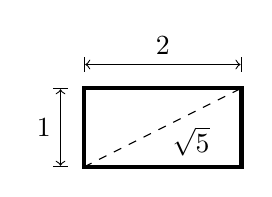
\begin{tikzpicture}
            \draw[ultra thick] (0,0) rectangle (2,1);
            \draw[|<->|] (-0.3,0) -- (-0.3,1) node[midway, anchor=east]{1};
            \draw[|<->|] (0,1.3) -- (2,1.3) node[midway, anchor=south]{2};
            \draw[dashed] (0,0) -- (2,1) node[midway, anchor=west, yshift=-5]{$\sqrt{5}$};
        \end{tikzpicture}
        \caption{A $1\times2$ rectangle.}
        \label{fig:rect-12}
    \end{subfigure}
    \begin{subfigure}[b]{.47\textwidth}
        \centering
        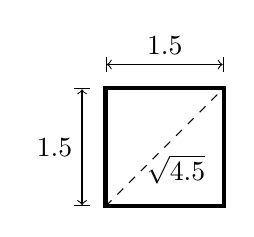
\begin{tikzpicture}
            \draw[ultra thick] (0,0) rectangle (1.5,1.5);
            \draw[|<->|] (-0.3,0) -- (-0.3,1.5) node[midway, anchor=east]{1.5};
            \draw[|<->|] (0,1.8) -- (1.5,1.8) node[midway, anchor=south]{1.5};
            \draw[dashed] (0,0) -- (1.5,1.5) node[midway, anchor=west, xshift=-10, yshift=-8]{$\sqrt{4.5}$};
        \end{tikzpicture}
        \caption{A $1.5\times1.5$ rectangle.}
        \label{fig:rect-15}
    \end{subfigure}
    \caption{}
    \label{fig:small-rects}
\end{figure}

Consider the $1\times2$ rectangles in figure \ref{fig:checker}. Since we have six $1\times2$ rectangles, six points, and at most one point per $1\times2$ rectangle, we must have exactly one point per $1\times2$ rectangle.

Also notice that any pair of adjacent $1\times1$ squares form a $1\times2$ rectangle. This means that no two points are in adjacent squares; otherwise, they would be in the same $1\times2$ rectangle. 

\begin{figure}[ht]
    \centering
    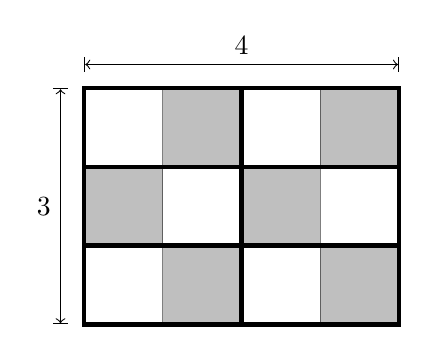
\begin{tikzpicture}
        \foreach \x/\y in {0/1, 1/0, 1/2, 2/1, 3/0, 3/2} {
            \draw[line width=0, fill=gray, opacity=0.5] (\x,\y) rectangle (\x+1,\y+1);
        }
        \draw[ultra thick] (0,0) rectangle (4,3);
        \draw[|<->|] (-0.3,0) -- (-0.3,3) node[midway, anchor=east]{3};
        \draw[|<->|] (0,3.3) -- (4,3.3) node[midway, anchor=south]{4};
        
        \draw[ultra thick] (0,1)--(4,1) (0,2)--(4,2) (2,0)--(2,3);
        
    \end{tikzpicture}
    \caption{The $3\times4$ rectangle partitioned into\\ twelve $1\times1$ squares and six $1\times2$ rectangles.}
    \label{fig:checker}
\end{figure}

Consider the $1\times2$ rectangle in the lower left. The point in this rectangle is either in the white square or the black square. Suppose the point is in the white square; this would mean that no point could be in the black square above this white square. So the point in the middle left rectangle would have to be in its respective white square. Following this reasoning, we find that all the points would need to be in white squares. Similarly, if we suppose the point in the lower left rectangle is in the black square, we find all the points to be in black squares.

Since the black and white regions are horizontal reflections of each other, we may assume, without loss of generality, that all the points are in white squares. More specifically, we have that each white square contains exactly one point.


\begin{figure}[ht]
    \centering
    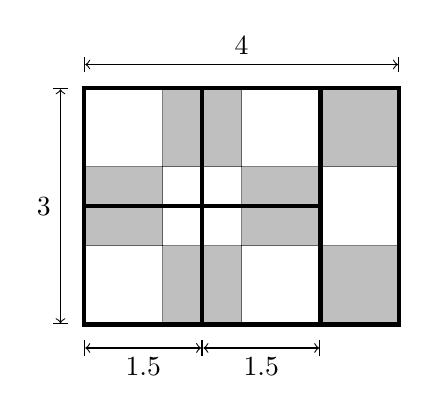
\begin{tikzpicture}
        \foreach \x/\y in {0/1,1/0,1/2,2/1,3/0,3/2} {
            \draw[line width=0, fill=gray, opacity=0.5] (\x,\y) rectangle (\x+1,\y+1);
        }
        \draw[ultra thick] (0,0) rectangle (4,3);
        
        \draw[ultra thick] (0,1.5) -- (3,1.5) (1.5,0) -- (1.5,3) (3,0) -- (3,3);
        
        
        \draw[|<->|] (-0.3,0) -- (-0.3,3) node[midway, anchor=east]{3};
        \draw[|<->|] (0,3.3) -- (4,3.3) node[midway, anchor=south]{4};
        \draw[|<->|] (0,-0.3) -- (1.5,-0.3) node[midway, anchor=north]{1.5};
        \draw[|<->|] (1.5,-0.3) -- (3,-0.3) node[midway, anchor=north]{1.5};
        
    \end{tikzpicture}
    \caption{The $3\times4$ rectangle partitioned into\\ four $1.5\times1.5$ squares and one $1\times3$ rectangle.}
    \label{fig:checker-15}
\end{figure}

Consider, now, the partitioning shown in figure \ref{fig:checker-15}. On the right, we have a single white square, and therefore point, in the $1\times3$ rectangle. The other five points must be elsewhere in the $3\times4$ rectangle. The rest of the rectangle is split into four $1.5\times1.5$ squares. With five points and four squares, we must have at least two points which are in the same $1.5\times1.5$ square. However, as previously shown, we cannot have two points in the same $1.5\times1.5$ square. This is a contradiction, so our original assumption must be false. Therefore, at least two points are at most $\sqrt{5}$ units apart.


\section*{Problem 16}
\fbox{
    \parbox{\textwidth} {
        A chess master who has 11 weeks to prepare a tournament decides to play at least one game every day but, in order not to tire himself, he decides not to play more than 12 games during any calendar week. Show that there exists a succession of (consecutive) days during which the chess master will have played exactly 21 games. (Hint: call $a_i$ the number of games that the chess master played the first $i$ days and consider the sequence $\{a_1, a_2, \dots, a_{77}, a_1+ 21, \dots, a_{77} + 21\}$.)
    }
}
\\

We will take $a_i$ to be the number of games the chess master has played the first $i$ days. We now consider the sequence $\{a_1, a_2, \dots, a_{77}, a_1+ 21, \dots, a_{77} + 21\}$.

Since the chess master plays at most 12 games per week, over 11 weeks, he will play no more than 132 games overall. And with at least one game per day, for all elements in the sequence $a_i$, we know $1\leq a_i \leq 132+21=153$.

With 154 elements in the sequence, each taking on some value from 1 to 153, at least two elements must be equal. Let $x,y$ be two such distinct elements. It is either the case that $x=a_i$ or $x=a_i+21$ for some $a_i$. Similarly, either $y=a_j$ or $y=a_j+21$ for some $a_j$. If $a_i=x=y=a_j$, then $x$ and $y$ would be the same day, since no two days have the same value. Similarly for if $a_i+21=x=y=a_j+21$. 

Without loss of generality, assume $x=a_i+21=a_j=y$. This means that in the days from $a_{i+1}$ to $a_j$, the chess master played exactly 21 games. So there exists a succession of consecutive days during which the chess master played exactly 21 games.




\end{document}